\documentclass[12pt]{article}
\usepackage{amsmath,amsthm,amssymb,dsfont,polynom}
\usepackage[pdftex]{graphicx}

\graphicspath{{images/}}

\usepackage[margin = 1.0in]{geometry}
\usepackage{fancyhdr}
\usepackage{hyperref}
\pagestyle{fancy}
\lhead{Francis Pich\'e}

\thispagestyle{empty}


\newtheorem{problem}{Problem} 
\theoremstyle{definition} 
\newtheorem*{solution}{Solution}

\usepackage{listings}
\usepackage{color}

\definecolor{dkgreen}{rgb}{0,0.6,0}
\definecolor{gray}{rgb}{0.5,0.5,0.5}
\definecolor{mauve}{rgb}{0.58,0,0.82}

\lstset{frame=tb,
  language= Java,
  aboveskip=3mm,
  belowskip=3mm,
  showstringspaces=false,
  columns=flexible,
  basicstyle={\small\ttfamily},
  numbers=none,
  numberstyle=\tiny\color{gray},
  keywordstyle=\color{blue},
  commentstyle=\color{dkgreen},
  stringstyle=\color{mauve},
  breaklines=true,
  breakatwhitespace=true,
  tabsize=3
}


\begin{document}
\title{COMP 303 Study guide}
\author{Francis Pich\'e}
\date{\today}
\maketitle
\newpage
\tableofcontents
\newpage

\part{Introduction}
\section{Disclaimer}
These notes are curated from Professor Joseph Vybihal's COMP303 lectures at McGill University. They are for study purposes only. They are not to be used for monetary gain.
\section{About This Guide}
I make my notes freely available for other students as a way to stay accountable for taking good notes. If you spot anything incorrect or unclear, don't hesitate to contact me via Facebook or e-mail at \url{http://francispiche.ca/contact/}
\part{Writing Good Code}
Good code is:
\begin{itemize}
	\item Optimal (Time complexity and memory)
	\item Simple
	\item Correct
	\item Robust (Few crashes, good error handling etc.)
	\item Easy to read
	\item Is well documented
	\item Uses accepted engineering techniques.
\end{itemize}
\section{Strategies for Writing Good Code}
\subsection{Optimality}
To minimize memory usage we could:
\begin{itemize}
	\item Encode long strings of data (compressing)
	\item Re-calulate instead of store values (trade-off with speed)
	\item Check library overhead!
	\item Data structure overhead (graph has a lot more pointers than a linked list!)
\end{itemize}
To minimize time complexity:
\begin{itemize}
	\item Come up with a better algorithm (Improve big O)
	\item Store more things in RAM (rather than in a DB or over a network)
	\item Avoid nesting of pointers
	\item Avoid deep or unnecessary recursion 
\end{itemize}
\subsection{Simplicity}
Strategies for simplicity:
\begin{itemize}
	\item Good variable names (avoid single letters except for array index's)
	\item Don't use lots of variables when an array is more appropriate
	\item Use simpler data structures if possible
	\item Reduce the volume of code
	\item Limit line length
	\item Modularize the program
	\item Use algorithms that are well known if possible
\end{itemize}
\subsection{Correctness}
The only way to be somewhat sure that your program is correct is through rigorous testing. Some things are easier to test than others, and theres entire QA departments that specialize in testing. But with the rise of Agile, more and more standard Devs need to be good at testing.
\\ \linebreak
Some general ideas on testing:
\begin{itemize}
	\item 1 test per 1 function
	\item Test valid inputs
	\item Test invalid inputs
	\item Test edge cases
	\item Validate that the output is correct
\end{itemize}
There's a ton of material online about testing and I definitely recommend taking some time to learn about more in-depth testing methods than what is covered in this course. It's required in almost all dev jobs and it's a very valuable skill to have.

\subsection{Readability}
This comes from good indentation, spacing and general style of code. Most people know this implicitly so I won't go into detail. For examples see the lecture slides from Lecture 2. 

\subsection{Comments as documentation}
The first place documentation happens is on the code level. This is where you can remove any ambiguity or sources of confusion from your code for other developers (or even future you). While real projects require real documentation, and excessive comments can be a detriment to readability, more comments are generally better than not enough. Break down your complex algorithms into comment separated steps, or add side-notes on anything that could be confusing to another developer.

\section{Well Designed Objects}
A well designed object should be one that does not cause any "wut?" moments amongst a team of developers. Specifically:
\begin{itemize}
	\item Single class per file
	\item Single purpose
	\item Expose only essential information
	\item Support an API structure
	\item Follow appropriate inheritance methods
\end{itemize}
\subsection{Single Purpose}
A class should be used to represent an idea, concept or object (pun-intended), and nothing more. A student should only contain ideas directly relevant to a student. A \texttt{Car} class should not have information about busses or trucks.
\\ \linebreak
This ensures that someone using your class can quickly find out everything there is to know about your object in an intuitive way. If your Student class has information about apples buried inside somewhere, someone on your team would have a hard time finding that out.
\subsection{Restriction of Information}
This is done to ensure that the class will be used correctly. There should be a decent amount of thought put into which parts of the code are "internal" and "external" to the class, ie: what parts of the class does the program need easy access to?
\\ \linebreak
Any time you use the \texttt{public} keyword, you should be thinking twice about if it's truly needed.
\subsection{Encapsulation}
When you take the concepts of single purpose and restriction of information and put them together, you get \textit{encapsulation}. Essentially what this means is that your class should be it's own complete bubble. No code outside the class should do the same things as inside your class, nor should things outside affect the class in an uncontrolled way.
\subsection{Inheritance}
To avoid duplication of code, we use inheritance to relate objects. This way classes can share common elements and simplify our lives. For details on inheritance see my COMP250 guide.
\\ \linebreak
Note that private information from a parent is not visible t the child.
\\ \linebreak
To design inheritance well:
\begin{itemize}
	\item A parent is more general
	\item A child is more specific
\end{itemize}
\subsection{Pre \& Post Conditions}
To keep things coherent, if a parent object imposes a condition on data, the child should maintain this condition. For example if a parent object has the condition that \texttt{salary} $>$ \texttt{0} then the child should not violate this by overriding the condition with say, negative values. It could, however, override it with \texttt{salary} $>$ \texttt{10000}.
\\ \linebreak
This is known as a \textbf{rich} starting point. Another example of a rich starting point is using a library, or some sample code.
\\ \linebreak
THis might be an issue since you may be inheriting, importing or implementing more features than are really needed.
\subsection{Extending vs Wrapping vs Interfaces}
Extending is when a new class contains the parent but adds extra methods and variables. Allows for polymorphism (see 250 guide for more on that). 
\\ \linebreak
Interfaces are used when the classes implementing are not necessarily related, but share common methods. For example the \texttt{Iterable} interface can be implemented by say, a \texttt{Degree} class, which contains a list of courses. But also a \texttt{Queue} class which has nothing to do with degrees or courses conceptually. So this allows for polymorphism across multiple inheritance trees.
\\ \linebreak
Wrapping is not a formal construct in a language, but it is the idea of placing objects inside a "wrapper" class, to put objects together in a more abstracted way.
\\ \linebreak
A special case is \texttt{abstract base classes}. These cannot be instantiated and contain both implemented and non-implemented methods. They provide the inheritance properties of extending, with the templating of interfaces. 

\section{Object Identity \& Lifecycle}
All objects have an idenity,(a reference or anonymous) and a lifecycle. Their lifecycle depends on the language and how they are handled (in C/C++ you have to manually free them from memory, vs garbage collection)
\subsection{Referenced Obects}
This is when an object is created by assigning its instance to a variable. \texttt{Object o = new Object()}. In this way, when no variables remain that point to this object, it is garbage collected (in Java) or causes a memory leak (C/C++).
\subsection{Anonymous Objects}
These are objects without references. For example \texttt{fn(new Object())}. It is then assigned a reference in the scope of the function, or in the scope of the Object to which it was passed into. For example if you pass an object into the constructor of another object, if it is then assigned to a variable in the second object, it will die with the object it is inside of.
\subsection{Static vs Instance}
A static object (or variable) can exist only once. That is, it cannot be instantiated. There can be no direct communication between static and instance structures.
\\ \linebreak
The \texttt{C} version of this would be in the two different ways of creating structs. One where you give your struct a name at the end, vs if you instantiate it afterwards.
\section{Object Class and Class Class}
All objects in Java extend the Object class. I went in-depth with this in my 250 guide, but I'll summarize here.
\\ \linebreak
There are a few important methods that the Object class has.
\begin{itemize}
	\item \texttt{toString()}
	\item \texttt{equals(Object o)}
	\item \texttt{hashCode()}
	\item \texttt{clone()}
\end{itemize}
\subsection{Object.toString()}
Automatically called by many functions such as print statements. Overwrite this to change the string representation of your object. By default, it stores the name of the object, and a unique hexedecimal identifier.
\subsection{Object.equals()}
Since the \texttt{==} operator only checks if the addresses are the same (for reference types), using it with reference types often has strange results. It is therefore necessary to override the \texttt{Object.equals()} method to specify what it means for two objects to be equal. Are their attributes equal?(This is the default) Etc. Note that the default will not look at nested Objects, so you must specify an equals method for complicated data structures.

\subsection{Object.hashCode()}
Hash data structures are only as good as their hash function. So if the default for your data type is really bad, so you'd have to implement your own hash function (override the hashCode() method.)

\subsection{Object.clone()}
The default clone makes a shallow copy by only cloning the references. (The contents of the original can be changed by the clone!!). A deep copy would be making a clone of all references and make them point to actual independent locations. This can be done with the clone() method.

\subsection{Type Inquiry}
This is the idea of testing what type a variable is. This is done using the \texttt{instanceof} operator. For example: \texttt{x isinstance Shape}.
\\ \linebreak
However, it does not check if it is exactly that type, it instead checks if \texttt{x} is part of the inheritance tree of Shape. We can use this to check if a cast will be successful.
\\ \linebreak
We can check for exact class matching with the \texttt{Object.getClass()} method. It returns an Object containing the type information for a class. This object contains the name, and a pointer to the superclass object. (The class object of it's parent).
\\ \linebreak
The Class class has some other useful methods such as \texttt{isArray()} and \texttt{getComponentType()} which 1) tests if the class is array, and 2) if it is, get the type of the components of the array.

\section{Reflection}
This is the practice of a program analyzing itself.
\\ \linebreak
The Class class we looked at is useful for reflection.
\\ \linebreak
We also have:
\begin{itemize}
	\item Class
	\item Package
	\item Field
	\item Method
	\item Constructor
	\item Array
\end{itemize}
Using these, we can get all the features of a class.
\begin{lstlisting}
Class super = Rectangle.class.getSuper();

Class[] interfaces = Rectangle.class.getInterfaces();

Package p = String.class.getPackage();

Field[] fields = Math.class.getDeclaredFields();
for (Field f: fields){
	if(Modifier.isStatic(f.getModifiers()))
}

Contstructor[] constructors = Rectangle.class.getDeclaredConstructors();

for(Constructor c: constructors){
	Class[] params = c.getParameterTypes(); // can be used on methods too!
Method m = PrintStream.class.getDeclaredMethod("println", String.class);
m.invoke(System.out, "Hello, world!"); //invoke is only for public methods
}

\end{lstlisting}
Note that we might get some errors with \texttt{getDeclaredMethod()} namely, \texttt{NoSuchMethodException},
\texttt{IllegalAccessException} , and 
\texttt{InvocationTargetException} 
\\ \linebreak
We can then use the \texttt{setAccessible(bool tf)} method on Fields to set the field to be able to modified. We can then use \texttt{set()} and \texttt{get()} on the fields.
\\ \linebreak
In this example, we'll resize an array:
\begin{lstlisting}
Object newA = Array.newInstance(a.getClass().getComponantType(), 2*Array.getLength(a) + 1);

System.arraycopy(a, 0, newA, 0, Array.getLength(a));

a = newA;
\end{lstlisting}

\section{Generic Types}
A generic type is instantiated when an actual type is substituted for the type-variable.
\\ \linebreak

\begin{lstlisting}
public class ArrayList<E>{
	public E get(int i){...}
}
\end{lstlisting}
If a type is used, it must always be the same for the same type variable. So if you give \texttt{E} a String, all references to \texttt{E} must be with a String.
\\ \linebreak
We can take this further, with extending. For example:
\begin{lstlisting}
public static <E, F extends E> void append(ArrayList<E> a, ArrayList<F> c){...}
\end{lstlisting}
So this would only allow types E and F if F extends E.
\\ \linebreak
Going \textit{even further} we can use wildcards like this:
\begin{lstlisting}
public static <E> void append(ArrayList<? super F> a, ArrayList<F> b, int count){...}
\end{lstlisting}
To say that anything which is a parent of F is valid.
\\ \linebreak
It's worth noting that all this stuff with generics is really just for the compiler and is an abstraction. The hardware doesn't care, and actually once the code is compiled, everything is an Object. Due to this, all Generics are just Objects when you try to do type inspection on them at runtime.
\\ \linebreak
Generics can't:
\begin{itemize}
	\item Throw or catch generic types.
	\item Use primitives
	\item Be static
	\item Be instantiated
	\item Mess up inheritance
\end{itemize}

\section{Specifications}
A specification is a written document from the designer to the programmer specifying the exact requirements for the project.
\\ \linebreak
They usually include:
\begin{itemize}
	\item User interface
	\item Input and Output
	\item Files and databases
	\item Objects, data structures, algorithms
	\item Features/functionality
	\item Menus, GUI's etc.
\end{itemize}
They are hard to write. They have to cover all cases, be clear, be what the client wants, and limiting assumptions.
\\ \linebreak
How can we use the compiler to enforce specifications?
\\ \linebreak
\subsection{Design by Contracts}
An interface can be used as a contract to enforce specifications.
\\ \linebreak 
Note that a class can implement multiple interfaces, and an interface can extend another interface.
\\ \linebreak
However this doesn't contain any information about how the methods should be implemented, this is what the document is for.
\\ \linebreak
When we do this, we could have something like \texttt{SomeInterface x = new SomeClassThatImplemented()}. The type of the variable dictates which methods can be called. (Methods that are in the class but not the interface cannot be accessed).

\section{Anonymous Objects and Classes}
As mentioned in a previous section, we can create objects without assigning them to a variable. This is useful for passing it into a method, which forces it to be garbage collected at the end of the method. Or, for passing into the constructor of another object, so that when the new object is destroyed, both will be destroyed.
\\ \linebreak
We can also write an anonymous class directly in the instantiation of an object!
\begin{lstlisting}
	
	Example<Object> ex = new Example<>(){
		public int compare(Example e1, Example e2){
			return e1.compareTo(e2)
		}
	}
\end{lstlisting}
When doing this, the class is tied to exactly one object. When the object is garbage collected, so is the class.
\\ \linebreak
Even crazier, we can make a method, which will generate new anonymous classes!
\begin{lstlisting}
public class Country{
	public static Comparator<Country> comparatorByName(){
		return new Comparator<Country>(){
			public int compare(Country c1, Country c2){
				return c1.getName().compareTo(c2.getName());
			}
		};
	}
}
\end{lstlisting}

\part{Aside: Swing GUI Programming}
I'll refrain from copy pasting the code from the slides here, but I'll do my best to provide the explanation that Prof. Vybihal gave in class.
\\ \linebreak

\section{Basic Structure}
The basic element of a GUI in swing as a \texttt{JFrame} object. This will cause the window to be displayed, and can be populated with elements.On this you can set a size, set a layout, (there are layout objects in Swing too, for example \texttt{GridLayout}). You can then add a listener to this frame to specify close, resize, minimize behaviors. (By implementing interfaces in an anonymous class).
\\ \linebreak
Next is the \texttt{JPanel} object. This is like the window, but is instead a canvas onto which elements are placed. This will be placed within the window. You can also give layouts to a panel, 
\\ \linebreak
To add buttons, we need to add listeners to our button elements. This is done by implementing the \texttt{actionPerformed} method. This method take an \texttt{ActionEvent} object which has information about the event. 
\\ \linebreak

\section{Object Truth \& Writing Good Classes}
Classes and objects represent a logical entity, and so must always stay consistent with the context of that entity. Put another way, they are an analogy to real things, and so must be consistent with the analogy. If we have a class Student, we expect it to behave and contain things that a Student would have. 
\\ \linebreak
Truth is the idea that the objects instantiated from a class are consistent with the analogy of the class.
\\ \linebreak
If we use setters, getter and mutators, we must ensure that they preserve truth.
\\ \linebreak

A class is\textbf{invariant} when all objects of the class are always in a valid state. 
\\ \linebreak
This may be broken for a moment in time \textbf{during} a "fix" to maintain this valid state.
\\ \linebreak

This idea is similar to that of \textbf{cohesion}, in which all methods of a class should belong to the same abstraction or analogy. If the class is for Students, it doesn't have anything else.
\\ \linebreak
We also need to find a balance with convenience, since too much cohesion can make the classes hard to use. For example, \texttt{pop()} is not only a pop. It also returns a value, so it's really a \texttt{peek()} and a \texttt{remove()}.
\\ \linebreak
We should also name and program in a way that is intuitive and consistent.

\section{Defensive Programming}
Always assume people are going to break your stuff. We must then validate all inputs and outputs.
\\ \linebreak
We do this using a \textbf{precondition} and \textbf{postcondition}. We use the precondition to test the inputs, do some work assuming everything is fine, and then validate the result at the end. Usually we can just use one, (usually preconditions because it saves work of doing the method).
\\ \linebreak
We throw exceptions when the expectation of the result is not obeyed. (If one of the conditions fails.) We only return if the result and inputs were valid. 

\part{Tools That Aid Good Design}
\section{Unit Testing}
A unit is a single "functioning unit", that is, it has no specific size or shape. It could be one method, a class, or collection of classes. We then cover this unit by handling all possible cases.
\\ \linebreak
We've already covered writing unit tests without tools in the earlier part of the course.
\\ \linebreak

\section{JUnit}
JUnit is a java framework for unit testing. It basically looks for classes and methods with the name "test" in them, and runs all your tests. 
\\ \linebreak
You would normally create a test class \texttt{DayTest} for example, that extends \texttt{TestCase}, a JUnit parent class. This parent class contains all the JUnit "stuff". 
\section{Javadoc}
The importance of documentation is self-evident. Javadoc is a tool that auto-generates an HTML file based on specially formatted comments in your code. They always begin with \texttt{/**} (rather than just /*). We then use the @ symbol to specify attributes. (for example: @author Francis Pich\'e, @return int) 
\\ \linebreak
Since it gets converted to HTML, you can actually inject html into the comments to add custom formatting!

\part{Modeling}

Software design is the idea of planning before coding. Abstractions and architecture are used to create a full model before beginning the implementation.
\\ \linebreak
The development (which would be done by the programmers) is controlled by the designer by using effective communication, strong OO constructs, and unit testing. The requirements are described by contracts, generalized code and UML (or some other modeling method). 
\\ \linebreak

\section{UML Class Diagrams}
This diagram describes all classes, data structures, objects and what they contain. 
\\ \linebreak
You could exhaustively go and model every possible attribute, method etc. But this is really hard to do since it's almost impossible for a designer to forsee every method a programmer would need, without writing anything himself. 
\\ \linebreak
In this class, we will make minimal diagrams, where we specify only the minimal variables and methods.
\\ \linebreak
You could also make hybrid responsibility diagrams, where instead of specifying methods you would write a "responsibility" description. (Not done in this course)
\\ \linebreak
A basic class would look like:
\\
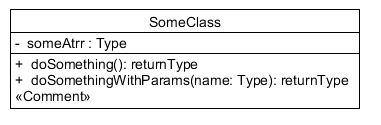
\includegraphics{basic_class}
\\
Where the + means public and the - means private.
\\ \linebreak
\subsection{Relations}
Since classes often depend and use each other, we need a way to depict this.
\\ \linebreak
\begin{itemize}
	\item Association : class A calls a method in class B
	\item Inheritance : A extends B
	\item Realization / Implementation : A implements B  
	\item Dependency : A assumes something about B but doesn't use it directly.
	\item Aggregation : see below
	\item Composition : see below
	\item Undirected : Relation in an undefined way.
\end{itemize}
Aggregation and composition are a little weird to understand. (At least for me!) Class A aggregates class B, if class B can exist without the existence of class A. Meanwhile, Class A composes class B if class B cannot exist without being within class A. \url{https://www.visual-paradigm.com/guide/uml-unified-modeling-language/uml-aggregation-vs-composition/}
\\ \linebreak
These relationships are expressed with these arrows: (in order)\\
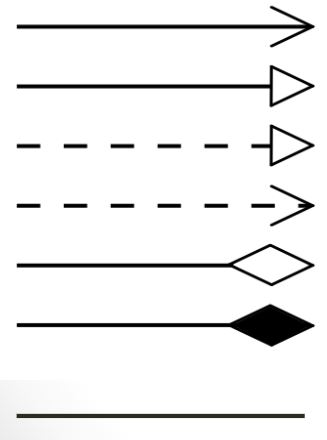
\includegraphics[scale=0.5]{arrows}
\\
Note that having TONS of arrows is probably a good indication of bad design.
\\ \linebreak
We can also express multiplicity by adding $n..m$ or $0..*$ etc. To show there should be between $n$ to $m$ instances, or $0$ to $\infty$ instances.
\\ \linebreak
\subsection{Examples}
\subsubsection{House}
	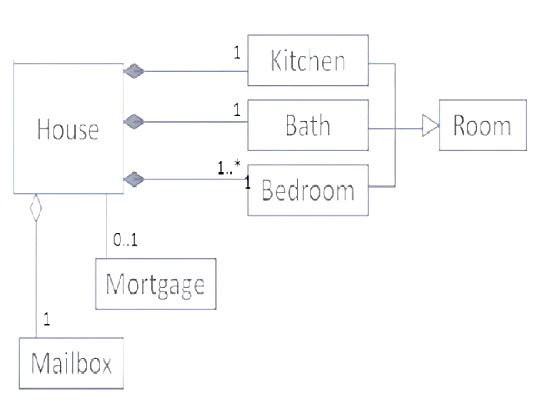
\includegraphics[]{house}
	\\
	The main method is most likely inside House, since most instantiations are coming out of house.
	\\ \linebreak
	In this picture, a House must have exactly 1 Kitchen, 1 Bathroom, and 1 to many Bedrooms. All of those extend Room. A Mortgage is somehow related, and can exist or not. A Mailbox is given to the house, but not necessarily part of it. (aggregation).
	\\ \linebreak
	There is actually a problem with this. Is Mailbox static? If not, then it must be instantiated by something. But this picture says it must be static, but it's also associated to the House using an aggregation, which means it must be instantiated.
	\\ \linebreak
	We could make this correct by adding another Main class which instantiates Mailbox (and possibly House if we don't want it to be static).
	\textbf{Always think of what needs to be instantiated!!!}

\subsubsection{University}
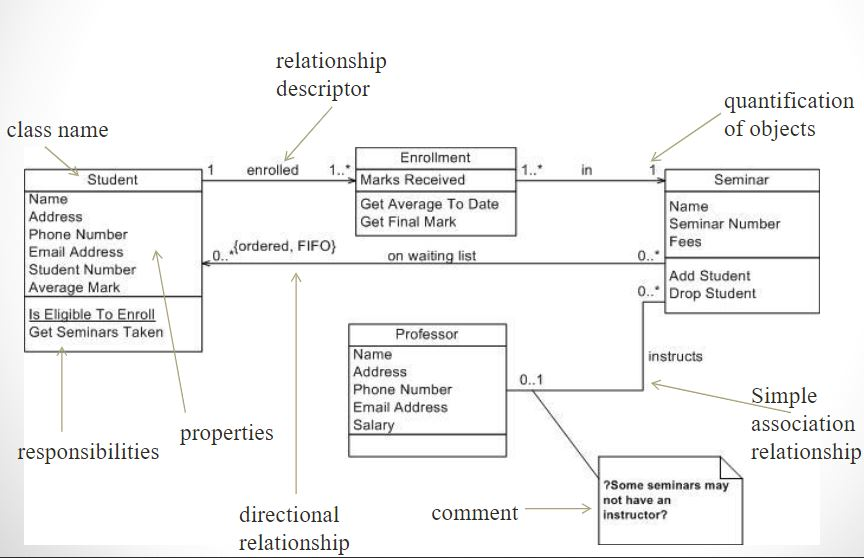
\includegraphics[]{university}
\\
Here we are adding labels to the associations. These describe what the relationship actually is. 
\\ \linebreak
Notice that Professor has no methods, since they aren't important and we are doing a hybrid responsibility here (even though we said we wouldn't do those!). Meanwhile, Enrollment has some methods since they are important to understanding the situation and requirements.
\\ \linebreak

\section{Sequence Diagram}
This is a use-case view of the system. Here we look at (in detail) what one part of the system will do in order. Very narrow and explicit.
\\ \linebreak
A class diagram does not explain the order (sequence) in which the program executes.
\\ \linebreak
In these we have a "timeline" representing execution flow, from left to right. The dotted lines coming down vertically break up the timeline into pieces by class. If the line is dotted the whole way down, the class is not executing, if there is a box, the class is executing. Solid arrows mean a method is being called, dotted arrows mean a value is being returned.
\\ \linebreak
We can add actors, who initiate the use cases.
\\ \linebreak
Loops and alternates are used to represent "for, while" and "or" (do not think about it as an if statement, since its not specified what the condition is.)
\\ \linebreak

\section{Activity Diagram}
Is essentially a flow chart of that the program should do. It can be for a single method, or a use case.
\\ \linebreak
This is more abstract and general than the sequence diagram, since it does not contain actual return values and methods, just plain words to describe whats happening.
\\ \linebreak
Note that there can be only one starting point, and can be many end points. 
\\ \linebreak
We can also make a multi-actor and object diagram, where we break up the diagram into columns of groups, and then individual actors. All actions regarding that actor fall within its column.

\part{Design Patterns}
The point of design patterns is to have a way of documenting language agnostic solutions to common software engineering problems. Often this is represented in UMl.
\\ \linebreak
A design pattern contains:
\begin{itemize}
	\item Title
	\item Long description of the problem
	\item Full description of the solution using UML
\end{itemize}

\section{Composite Pattern}
From the wiki:
\\ \linebreak
"A part-whole hierarchy should be represented so that clients can treat the part and whole objects uniformly."
\\ \linebreak
Basically, one object contains a list of others which implement a common interface so that they can be called together.
\\ \linebreak
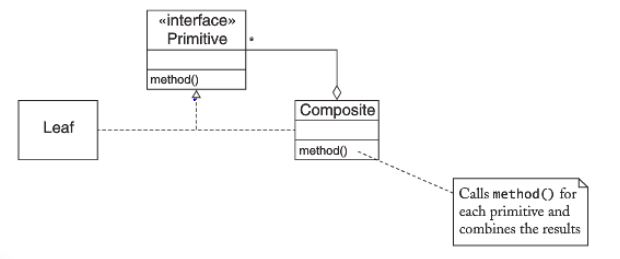
\includegraphics{composite}
\\
Here, both Leaf and Composite implement the Primitive interface. The method() of Composite simply calls the method() of all the Leaves which it contains. 
\\ \linebreak
This can be used to allow for individual Leaf objects to call method() by themselves, or be part of some greater Composite, and be called together.
\\ \linebreak
Example:
\begin{lstlisting}

class Team implements CompositeInterface{
	private ArrayList<T> team = new ArrayList<S>(); //Generic 
	public void deductHitPoint(int n){
		for(T member : this.team){
			member.deductHitPoint(n);
		}
	}
}

class Soldier implements SoldierInterface{
	private float hp;
	public void deductHitPoint(int n){
		this.hp -= n;
	}
}

interface CompositeInterface{
	public void deductHitPoint(int n);
}
\end{lstlisting}

\section{Decorator Pattern}
Suppose we want to add a feature to a method in an existing class. We use a decorator to add functionality.
\\ \linebreak
In Java we can write a new method, override or simply overwrite. This is different from a wrapper since we are not wrapping a primitive, we are wrapping classes. When classes are wrapped, we do not call it wrapping.
\\ \linebreak
For example: Arrow and Magic Arrow should behave and be treated the same, except that Magic Arrow will have some extra functionality onto it.
\\ \linebreak

\end{document}